\documentclass{report}

\usepackage[utf8]{inputenc}
\usepackage[nottoc]{tocbibind}
\usepackage{vhistory}
\usepackage[ampersand]{easylist}
\usepackage{natbib}
\usepackage{url}
\usepackage{scrextend}
\usepackage{graphicx}
\usepackage{multicol}
\usepackage[titletoc]{appendix}
\usepackage{float}
\usepackage{blindtext}
\usepackage{listings}
\usepackage{xcolor}
\usepackage{tabto} \NumTabs{3}

\input {resources/alloyListing}

\graphicspath{ {img/} }

\begin{document}

\begin{titlepage}
	\centering
	
\includegraphics[width=0.5\textwidth]{polimi-logo}\par\vspace{1cm}
	{\scshape\LARGE Politecnico di Milano\par}
	\vspace{1cm}
	{\scshape\Large Software Engineering 2 project\par}
	\vspace{1.5cm}
	{\Huge\bfseries PowerEnJoy\par}
	\vspace{0.5cm}
	{\Large\bfseries Requirement Analysis and Specification Document\par}
	\vspace{2cm}
	\begin{multicols}{2}
		{\Large\itshape Matteo Penco\par}
		\vspace{0.25cm}
		mat. 875740
		\vfill\columnbreak
		{\Large\itshape Riccardo Pressiani\par}
		\vspace{0.25cm}
		mat. 874948
	\end{multicols}
	
	\vfill
	
	{\Large Version 1.0.1 approved\par}
	\vspace{1.25cm}
	{\large \today\par}
\end{titlepage}

\begin{versionhistory}
  \vhEntry{0.1}{26.10.16}{RP}{Document created}
  \vhEntry{1.0}{13.11.16}{RP and MP}{Document approved}
  \vhEntry{1.0.1}{14.11.16}{RP and MP}{Fix bug in Alloy model}
\end{versionhistory}

\vspace{5cm}
{\noindent\Huge\bfseries Hours of work\par}
\vspace{0.5cm}
{\noindent Matteo Penco	\tab{35h}\par}
{\noindent Riccardo Pressiani \tab{35h}\par}

\tableofcontents

%Introduction
\chapter{Introduction}

\section{Purpose}
This document provides a high detailed description about the design and the architecture of the PowerEnJoy software.
It includes the design information about the components and how they intereact among them, the design of the most complex algorithm and the user interface design of the software to be developed.

This document is inteded for the key design stakeholders, which include managers and the development team.

\section{Scope}
PowerEnJoy is inteded to be a management system for a car-sharing system that exclusively employs electrical powered cars.
The system allows users to find all the available cars near a given location which can be their current position or a specific address typed in. The user can book one of the cars available for a limited amount of time.
Once the booked car is reached by the user, it can be unlocked from one of the smart devices of the user. After entering a PIN, decided by the user during the registration phase, on the onboard computer, the engine can be started and the rental begins.
The cost of the service is calculated on the total duration of the rental multiplied by a fixed rate per minute. The user is continuously informed about the cost of the ongoing rental by the onboard computer.
The user can end the rental by parking the car and stopping the engine.

The PowerEnJoy platform is intended to be available on the major mobile devices, such as smartphones and tablets running iOS \cite{ios} or Android \cite{android}.
\section{Definitions, acronyms and abbreviations}

% \subsection{Definitions}
% 	\begin{labeling}{defs}
% 		\item[\textbf{TEST}] \blindtext
% 	\end{labeling}

\subsection{Acronyms}
	\begin{labeling}{acro}
		\item[\textbf{PIN}] Personal Identification Number
		\item[\textbf{RASD}] Requirement Analysis and Specification Document
	\end{labeling}

% \subsection{Abbreviations}
% 	\begin{labeling}{abbrv}
% 		\item[\textbf{TEST}] \blindtext
% 	\end{labeling}
\section{References}

\begin{itemize}
	\item Assigments document for the first semester project of the Software Engineering 2 course held at Politecnico di Milano by Mottola Luca and Di Nitto Elisabetta \cite{assignments}.
	\item PowerEnjoy - Requirement Analysis and Specification Document \cite{rasd}.
	\item IEEE Standard for Information Technology—Systems Design— Software Design Descriptions \cite{ieee_sdd}.
	\item IEEE Systems and software engineering — Architecture description \cite{ieee_arch}.
	\item IEEE Recommended Practice for Architectural Description of Software-Intensive Systems \cite{ieee1471}.
\end{itemize}

% !TEX root = ../../../main.tex

\section{Overview}

A general introduction about the PowerEnJoy project has been given in this chapter. In the following chapters the reader will be provided with a more detailed description of the integration testing procedures.

In Chapter 2, the entry criteria to begin the integration testing phase will be provided. Moreover, the strategy and the integration test order will be described.

In Chapter 3, a detailed description of each integration test will be provided. These descriptions will include the expected input values and the corresponding state after each method invocation.

In Chapter 4, tools and equipment used to perform the tests will be listed along with a brief description.

In Chapter 5, the drivers needed and the set of data used to perform the tests correctly will be described.


%Overall Description
\input{chapters/ch2/2-overall-description}
%Specific requirements
\input{chapters/ch3/3-specific-requirements}

\begin{appendices}
	%Scenarios and UML models
	\chapter{Scenarios and UML Models}
In this appendix are included some scenarios and UML models in order to provide graphical representations of some of the most complex processes of the systems.

\input{chapters/appendices/appendix-a/sections/a-1-scenarios}
\section{Use case model}

\begin{figure}[H]
	\centering
	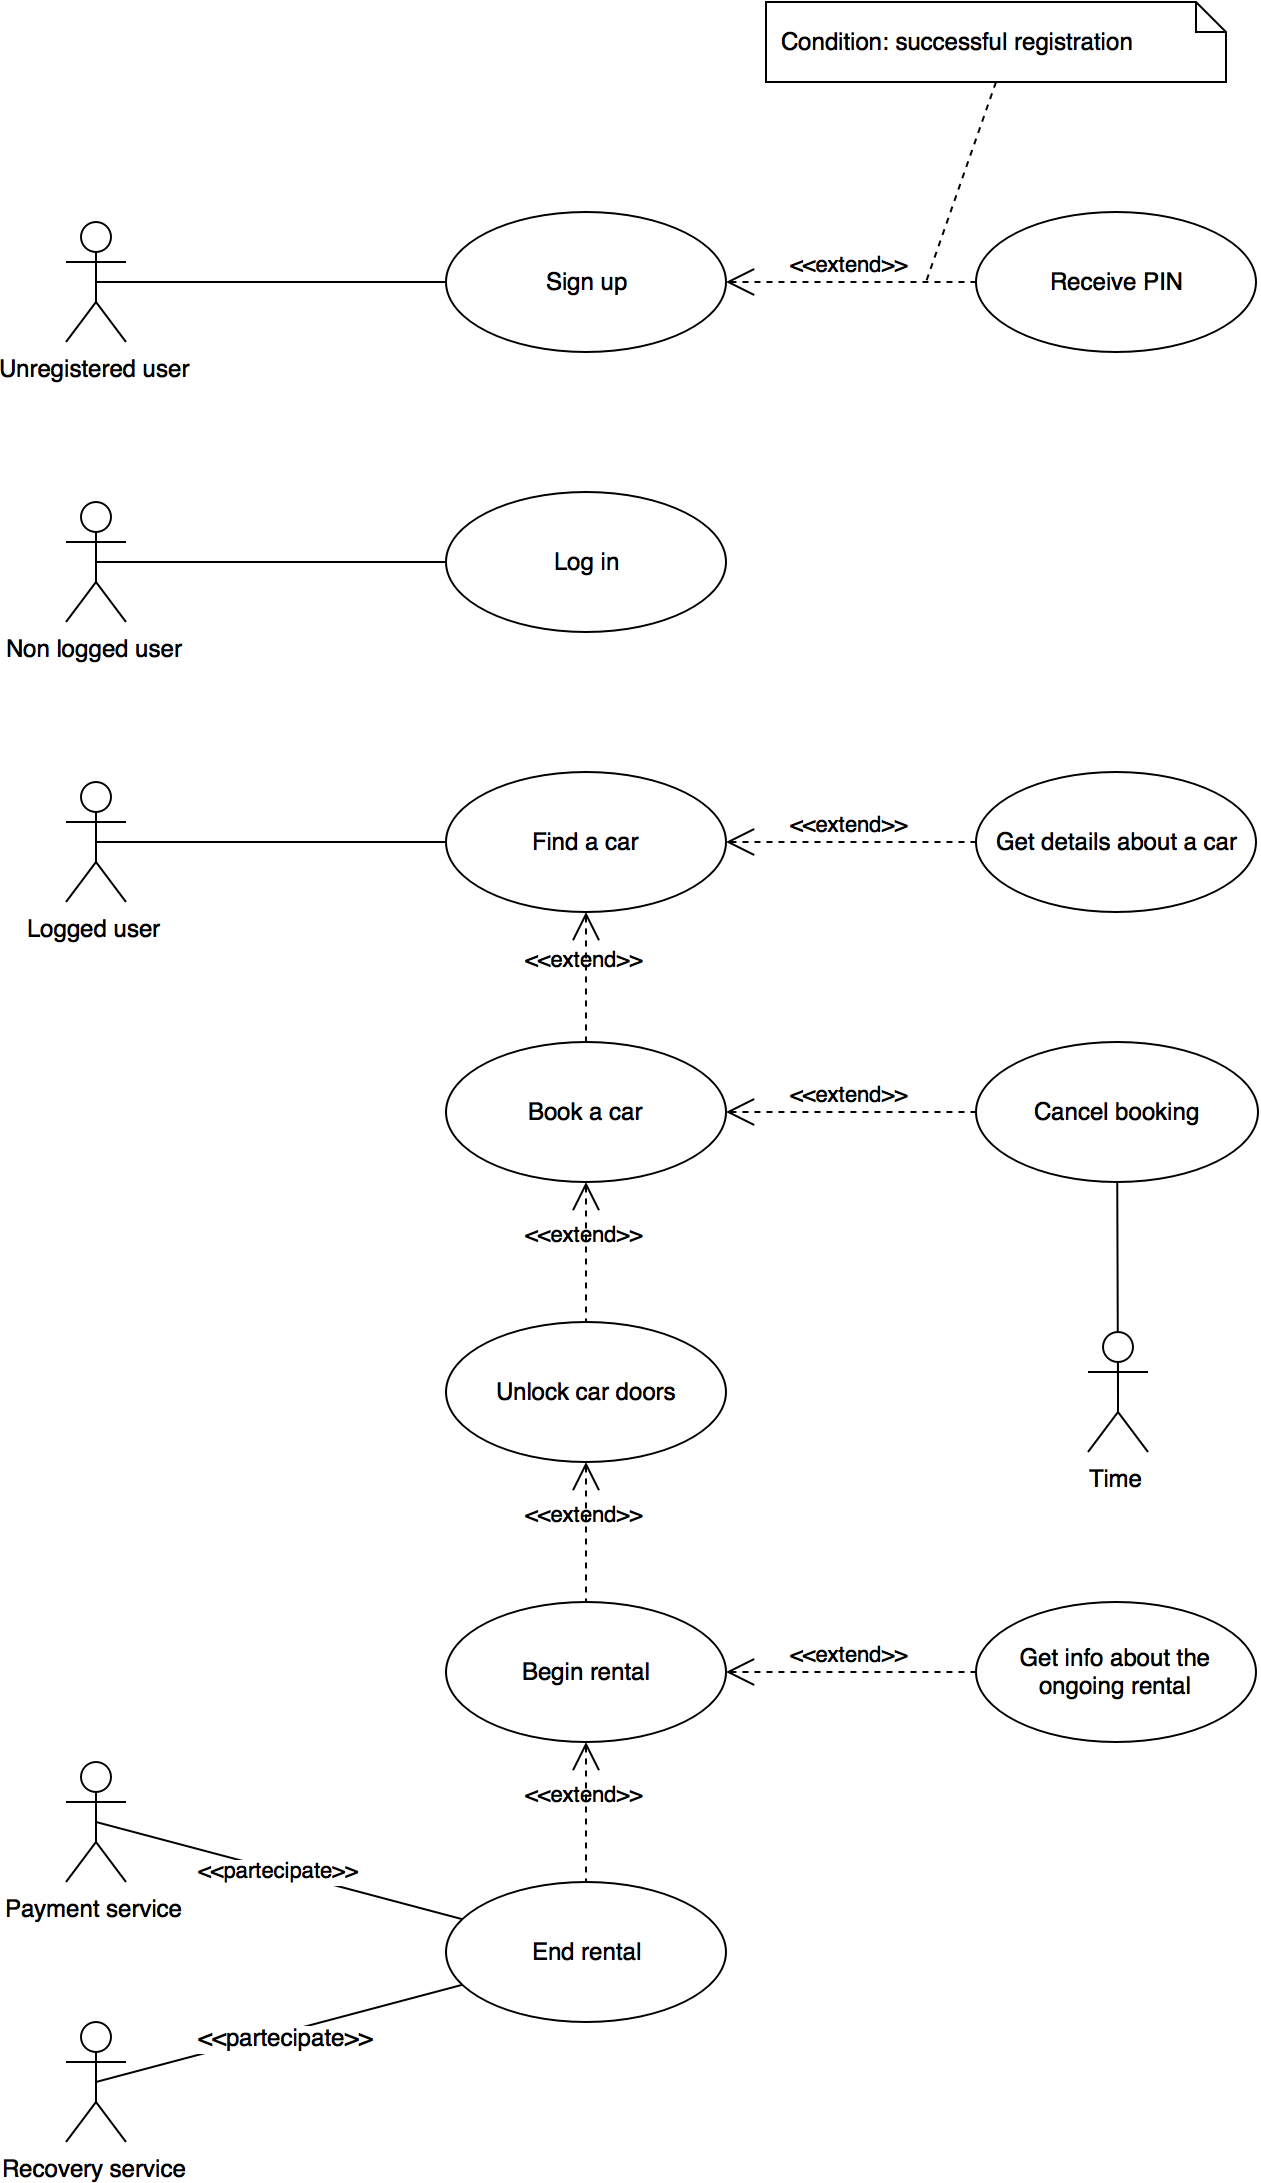
\includegraphics[width=0.8\textwidth]{use-case-model}
	\caption[Use case model]{The diagram above represents the use case model of the PowerEnJoy project. All the use cases are included along with the actors involved in their execution.}
	\label{fig:use-case-model}
\end{figure}

\subsection{Use case description 1 - Sign up}
\begin{labeling}{use-case-desc-1}
	\item[\textbf{Name}] Sign up
	\item[\textbf{Actors}] User
	\item[\textbf{Entry conditions}] There are no entry conditions.
	\item[\textbf{Flow of events}]
		\begin{itemize}
			\item[]
			\item The user accesses the homepage of PowerEnJoy or opens the app.
			\item The user inserts his/her credentials in the registration form.
			\item The user clicks on the sign up button.
			\item The system processes the registration of the user.
		\end{itemize}
	\item[\textbf{Exit conditions}] The user is successfully registered to the system.
	\item[\textbf{Exceptions}]
		\begin{itemize}
			\item[]
			\item Credentials provided by the user are not correct. In this case the system notifies the user of the error and let him/her to input again his/her credentials. 
			\item User is already registered. In this case the system notifies the user of the impossibility to register.
		\end{itemize}
\end{labeling}

\subsection{Use case description 2 - Receive the PIN}
\begin{labeling}{use-case-desc-2}
	\item[\textbf{Name}] Receive the PIN
	\item[\textbf{Actors}] User
	\item[\textbf{Entry conditions}] The user must have completed the registration.
	\item[\textbf{Flow of events}]
		\begin{itemize}
			\item[]
			\item The system generates the new PIN for the registered user
			\item The system sends to the registered user his/her PIN via mail
		\end{itemize}
	\item[\textbf{Exit conditions}] The user successfully receives the PIN to use PowerEnJoy cars.
	\item[\textbf{Exceptions}]
		\begin{itemize}
			\item[]
			\item The user doesn’t receive the PIN via mail. In this case the user can ask to the system to send again the mail with the PIN.
		\end{itemize}
\end{labeling}

\subsection{Use case description 3 - Log in}
\begin{labeling}{use-case-desc-3}
	\item[\textbf{Name}] Log in
	\item[\textbf{Actors}] User
	\item[\textbf{Entry conditions}] The user has to be already registered.
	\item[\textbf{Flow of events}]
		\begin{itemize}
			\item[]
			\item The user accesses the homepage of PowerEnJoy or opens the app
			\item The user inputs his email and password
			\item The user clicks on the log in button
			\item The system redirects the user on his personal page
		\end{itemize}
	\item[\textbf{Exit conditions}] The user is successfully redirected to his personal page.
	\item[\textbf{Exceptions}]
		\begin{itemize}
			\item[]
			\item Email or password provided by the user are not correct. In this case the system notifies the user of the error and let him/her to input again his/her credentials. 
		\end{itemize}
\end{labeling}
\begin{figure}[H]
	\centering
	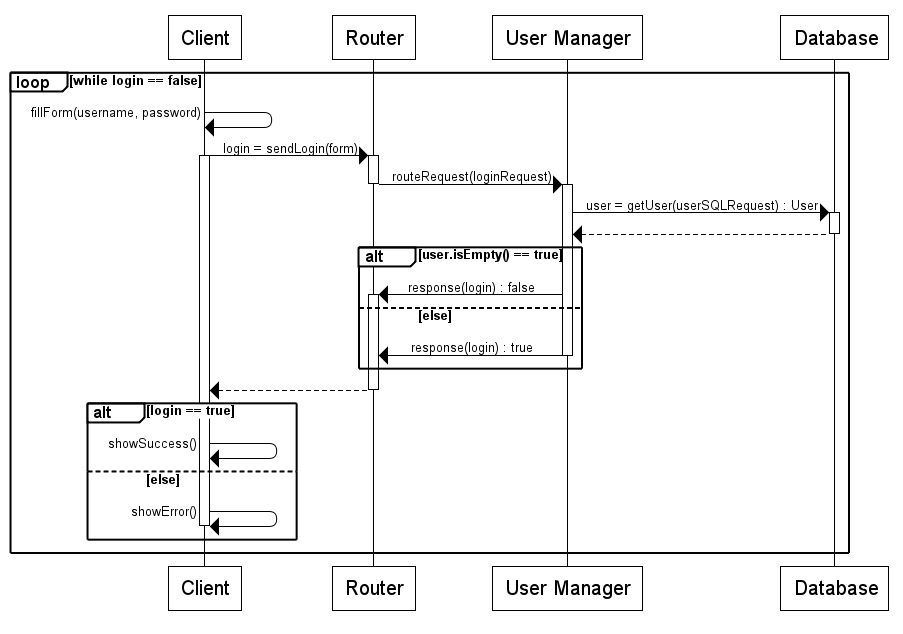
\includegraphics[width=\textwidth]{sequence-diagrams/login}
	\caption[Sequence diagram - Log in]{The sequence diagram above describes the log in procedure.}
	\label{fig:login-sequence-diagram}
\end{figure}
\clearpage

\subsection{Use case description 4 - Find a car}
\begin{labeling}{use-case-desc-4}
	\item[\textbf{Name}] Find a car
	\item[\textbf{Actors}] User
	\item[\textbf{Entry conditions}] The user has to be logged in.
	\item[\textbf{Flow of events}]
		\begin{itemize}
			\item[]
			\item The user inserts a specified address or chooses his current position
			\item The system loads on the map all available cars and all safe areas near the position provided by the user
		\end{itemize}
	\item[\textbf{Exit conditions}] The user can see on the map all available cars and all safe areas near the position provided. 
	\item[\textbf{Exceptions}]
		\begin{itemize}
			\item[]
			\item The user inserts an invalid address. In this case the system notifies the user of the error and let him/her to insert a new address.
			\item User’s GPS doesn’t work. In this case the system notifies the user of the impossibility to process the request.
		\end{itemize}
\end{labeling}

\subsection{Use case description 5 - Get details about a car}
\begin{labeling}{use-case-desc-5}
	\item[\textbf{Name}] Get details about a car
	\item[\textbf{Actors}] User
	\item[\textbf{Entry conditions}] The user must have looked for available cars on the map.
	\item[\textbf{Flow of events}]
		\begin{itemize}
			\item[]
			\item The user clicks on an available car shown on the map
			\item The system shows the details about the car chosen by the user
		\end{itemize}
	\item[\textbf{Exit conditions}] The user can see the details of the chosen available car.
	\item[\textbf{Exceptions}]
		\begin{itemize}
			\item[]
			\item Given the assumptions written below, there are no exceptions in this flow of events.
		\end{itemize}
\end{labeling}

\subsection{Use case description 6 - Book a car}
\begin{labeling}{use-case-desc-6}
	\item[\textbf{Name}] Book a car
	\item[\textbf{Actors}] User
	\item[\textbf{Entry conditions}] The user must have looked for available cars on the map.
	\item[\textbf{Flow of events}]
		\begin{itemize}
			\item[]
			\item The user clicks on an available car shown on the map
			\item The system asks the user if he/she wants to confirm the action
			\item The user clicks on the confirmation button
			\item The system confirms the booking of the chosen car and gives the opportunity to cancel the booking
		\end{itemize}
	\item[\textbf{Exit conditions}] The user successfully books a car.
	\item[\textbf{Exceptions}]
		\begin{itemize}
			\item[]
			\item Another user books a car before the user confirms the booking. In this case the system redirects the user on the map updated with the new situation of available cars.
		\end{itemize}
\end{labeling}
\begin{figure}[H]
	\centering
	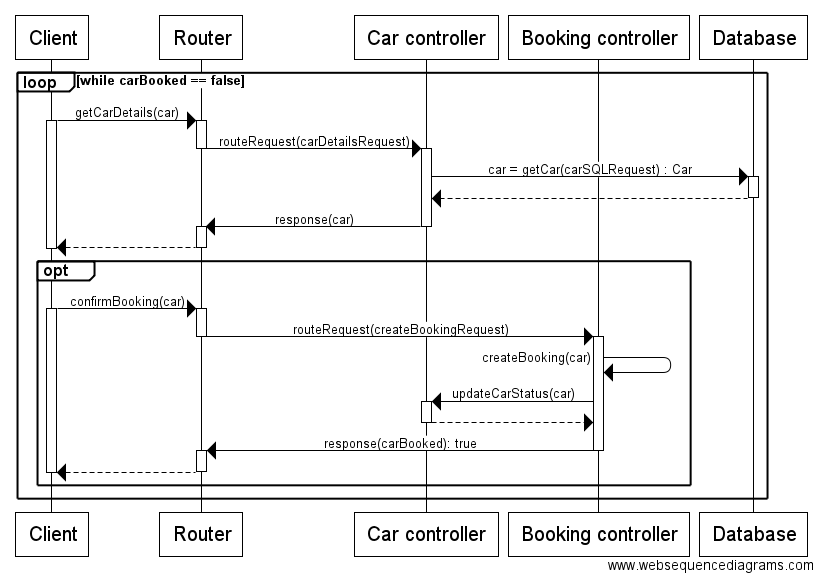
\includegraphics[width=0.7\textwidth]{sequence-diagrams/booking}
	\caption[Sequence diagram - Book a car]{The sequence diagram above describes the car booking procedure.}
	\label{fig:booking-sequence-diagram}
\end{figure}
\clearpage

\subsection{Use case description 7 - Cancel booking}
\begin{labeling}{use-case-desc-7}
	\item[\textbf{Name}] Cancel booking
	\item[\textbf{Actors}] User
	\item[\textbf{Entry conditions}] The user must have booked a car.
	\item[\textbf{Flow of events}]
		\begin{itemize}
			\item[]
			\item The user clicks on the button to cancel booking
			\item The system asks the user if he/she wants to confirm the action
			\item The system confirms the cancellation of booking
		\end{itemize}
	\item[\textbf{Exit conditions}] user successfully cancels booking of the car.
	\item[\textbf{Exceptions}]
		\begin{itemize}
			\item[]
			\item It passed an hour since the booking confirmation. In this case the system has already cancelled automatically booking. 
		\end{itemize}
\end{labeling}
\begin{figure}[H]
	\centering
	\includegraphics[width=0.6\textwidth]{sequence-diagrams/cancel-booking}
	\caption[Sequence diagram - Cancel booking]{The sequence diagram above describes the booking cancellation procedure.}
	\label{fig:cancel-booking-sequence-diagram}
\end{figure}
\clearpage

\subsection{Use case description 8 - Unlock car doors}
\begin{labeling}{use-case-desc-8}
	\item[\textbf{Name}] Unlock car doors
	\item[\textbf{Actors}] User
	\item[\textbf{Entry conditions}] The user must have booked a car.
	\item[\textbf{Flow of events}]
		\begin{itemize}
			\item[]
			\item The user is notified by the system that he's near enough to the booked car to unlock its doors
			\item The user clicks on the button to unlock the booked car
			\item The system unlocks car doors
		\end{itemize}
	\item[\textbf{Exit conditions}] The user successfully unlocks car doors.
	\item[\textbf{Exceptions}]
		\begin{itemize}
			\item[]
			\item It passed an hour since the booking confirmation after the system gave the possibility to the user to unlock car doors. In this case the user can't unlock car doors because the system has already cancelled automatically booking.  
		\end{itemize}
\end{labeling}
\begin{figure}[H]
	\centering
	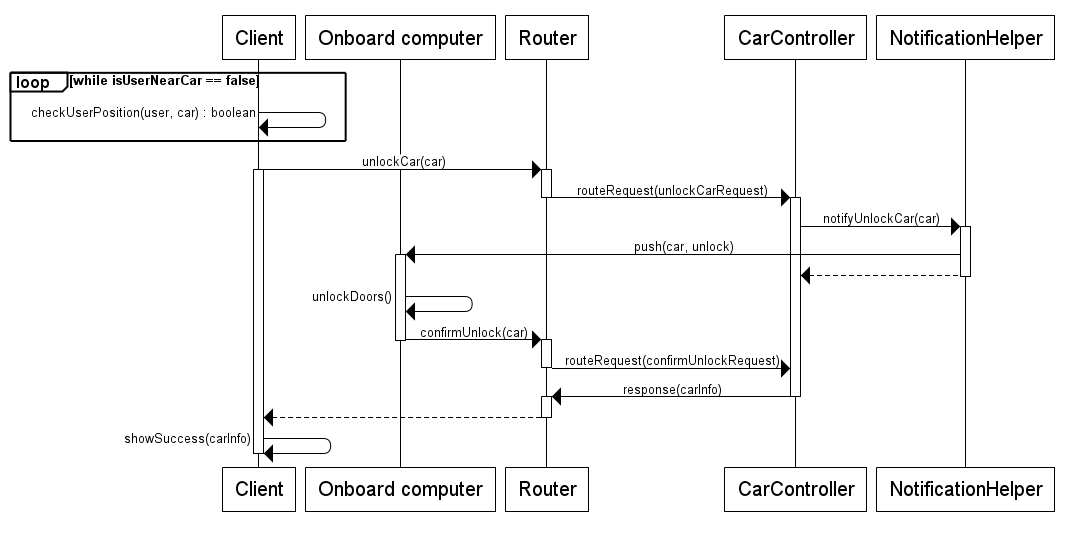
\includegraphics[width=0.8\textwidth]{sequence-diagrams/open-car}
	\caption[Sequence diagram - Unlock car doors]{The sequence diagram above describes the car doors unlocking procedure.}
	\label{fig:open-car-sequence-diagram}
\end{figure}
\clearpage

\subsection{Use case description 9 - Begin rental}
\begin{labeling}{use-case-desc-9}
	\item[\textbf{Name}] Begin rental
	\item[\textbf{Actors}] User
	\item[\textbf{Entry conditions}] The user must have unlocked car doors.
	\item[\textbf{Flow of events}]
		\begin{itemize}
			\item[]
			\item The user inserts the PIN provided at the moment of registration on the onboard computer of the car.
			\item The user ignites the engine.
		\end{itemize}
	\item[\textbf{Exit conditions}] The user starts driving the car.
	\item[\textbf{Exceptions}]
		\begin{itemize}
			\item[]
			\item The PIN inserted by the user is not correct. In this case the system doesn't allow the usere to ignite the engine until he inserts the correct PIN. 
		\end{itemize}
\end{labeling}
\begin{figure}[H]
	\centering
	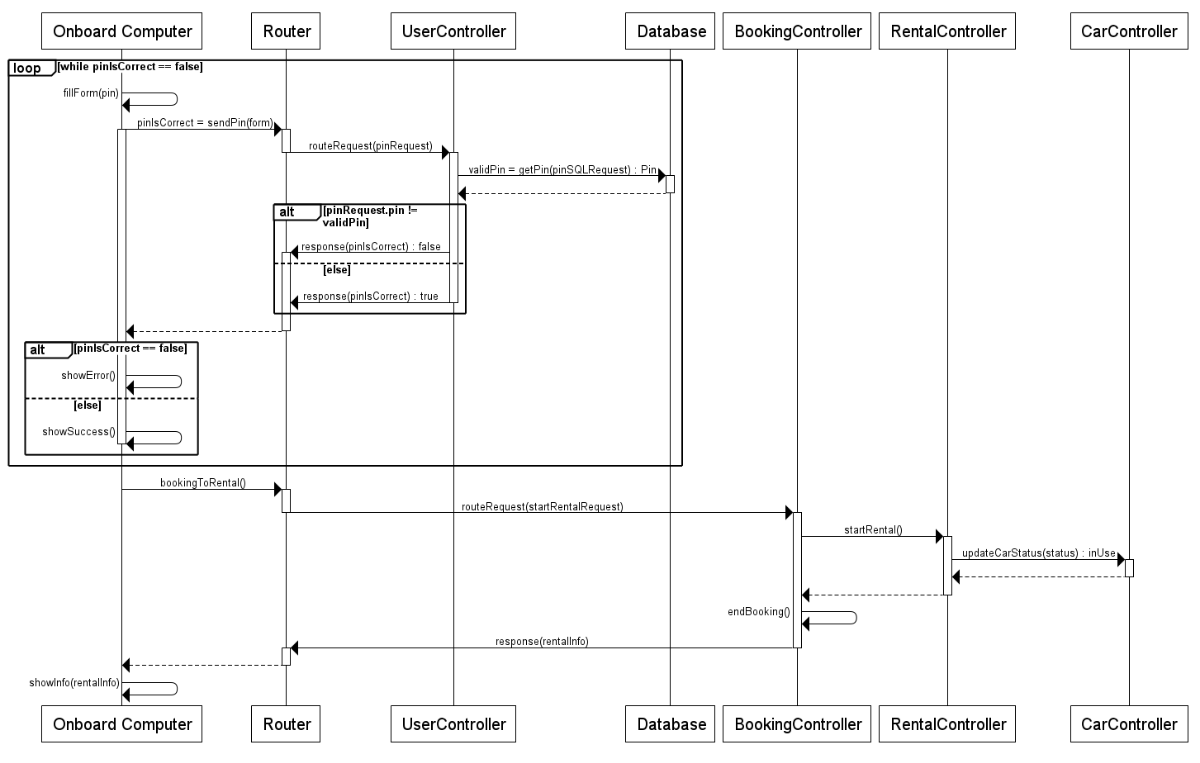
\includegraphics[width=0.8\textwidth]{sequence-diagrams/begin-rental}
	\caption[Sequence diagram - Begin rental]{The sequence diagram above describes the rental beginning procedure.}
	\label{fig:begin-rental-sequence-diagram}
\end{figure}
\clearpage

\subsection{Use case description 10 - Get info about the ongoing rental}
\begin{labeling}{use-case-desc-10}
	\item[\textbf{Name}] Get info about the ongoing rental
	\item[\textbf{Actors}] User
	\item[\textbf{Entry conditions}] The user must have started a rental.
	\item[\textbf{Flow of events}]
		\begin{itemize}
			\item[]
			\item The user interacts with the onboard computer interface in order to get information about the ongoing rental.
			\item The systems shows on the onboard computer the desired information.
		\end{itemize}
	\item[\textbf{Exit conditions}] The user successfully gets desired information about the ongoing rental. 
	\item[\textbf{Exceptions}]
		\begin{itemize}
			\item[]
			\item The car's battery runs out. In this case the onboard computer can't give any further information about the ongoing rental except the total cost of the rental reached before the battery exhausted. 
		\end{itemize}
\end{labeling}

\subsection{Use case description 11 - End rental}
\begin{labeling}{use-case-desc-11}
	\item[\textbf{Name}] End rental
	\item[\textbf{Actors}] User
	\item[\textbf{Entry conditions}] The user must have started a rental.
	\item[\textbf{Flow of events}]
		\begin{itemize}
			\item[]
			\item The user parks the car in a safe area.
			\item The user turns off the engine.
			\item The user and, eventually, passengers exit the car and close car doors.
		\end{itemize}
	\item[\textbf{Exit conditions}] The user successfully ends the rental.
	\item[\textbf{Exceptions}]
		\begin{itemize}
			\item[]
			\item The user parks the car non in a safe area. In this case the system doesn't allow the user to end the rental.
			\item The user parks the car in a safe area but doesn't turn off the engine. In this case the system doesn't allow the user to end the rental.
			\item The user parks the car in a safe area, turns off the engine but he/her and eventually passengers don't exit the car or close car doors. In this case the system doesn't allow the user to end the rental.  
		\end{itemize}
\end{labeling}
\begin{figure}[H]
	\centering
	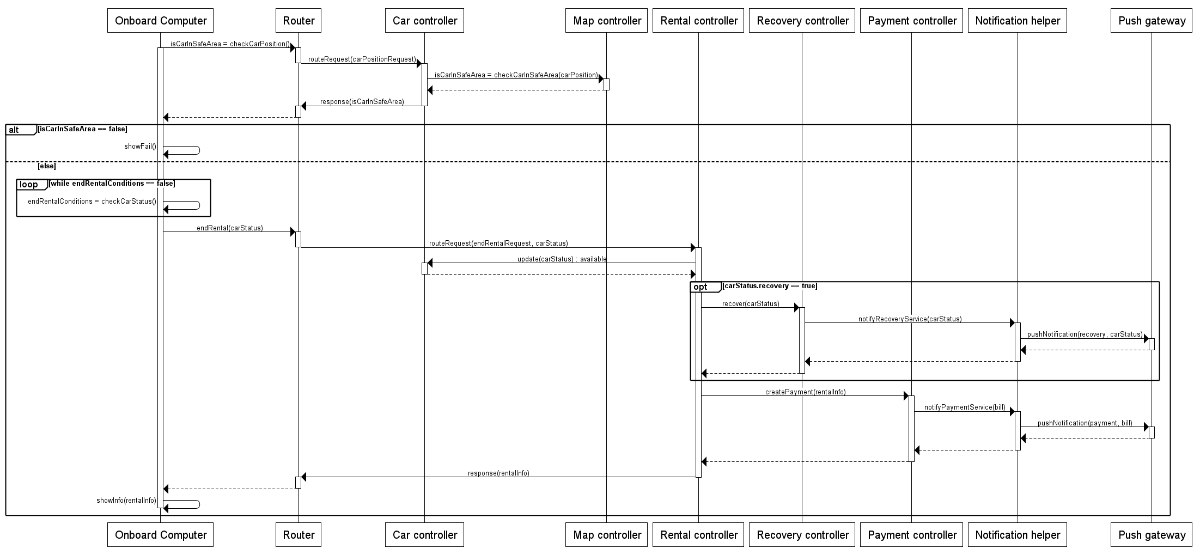
\includegraphics[width=\textwidth]{sequence-diagrams/end-rental}
	\caption[Sequence diagram - End rental]{The sequence diagram above describes the rental ending procedure.}
	\label{fig:end-rental-sequence-diagram}
\end{figure}
\clearpage

\input{chapters/appendices/appendix-a/sections/a-3-state-diagrams}
\input{chapters/appendices/appendix-a/sections/a-4-class-diagram}

	%Alloy
	\chapter{Alloy Model}
In this appendix a model of the PowerEnJoy system written in Alloy \cite{alloy} is provided.

\input{chapters/appendices/appendix-b/sections/b-1-signatures}
\newpage

\section{Facts}

\lstset{language=alloy}

\begin{lstlisting}
fact carsAreUnique {
	all c1, c2: Car | (c1 != c2) => c1.IDCar != c2.IDCar
}

fact positionsAreUnique {
	all p1, p2: Position |
		(p1 != p2) => (p1.latitude != p2.latitude) ||
		(p1.longitude != p2.longitude)
}

fact carsCannotBeInTheSamePlace {
	all c1, c2: Car | (c1 != c2) => (c1.position != c2.position)
}

fact safeAreaAreUnique {
	all s1, s2: SafeArea | (s1 != s2) => (s1.position != s2.position)
}

fact usersAreUnique {
	all u1, u2: User | (u1 != u2) => (u1.taxCode != u2.taxCode)
}

fact bookingsAreUnique {
	all b1, b2: Booking | (b1 != b2) => (b1.bookingID != b2.bookingID)
}

fact oneCarOneBooking {
	all b1, b2: Booking |
		(b1.ended = False && b2.ended = False && b1.car = b2.car) => (b1 = b2)
}

fact oneUserOneBooking {
	all b1, b2: Booking |
		(b1.ended = False && b2.ended = False && b1.user = b2.user) => (b1 = b2)
}

fact rentalIfNotElapsed {
	all r: Rental | r.booking.elapsedTime = False
}

fact oneBookingOneRental {
	all r1, r2: Rental | (r1 != r2) => r1.booking != r2.booking
}

fact feeIfElapsed {
	all p: PaymentFee | p.booking.elapsedTime = True
}

fact endBookingIfElapsed {
	all p: PaymentFee | p.booking.ended = True
}

fact paymentFeeAreUnique {
	all p1, p2: PaymentFee | (p1 != p2) => (p1.booking != p2.booking)
}

fact paymentRentalAreUnique {
	all p1, p2: PaymentRental | (p1 != p2) => (p1.rental != p2.rental)
}

fact payIfRentalEnded {
	all p: PaymentRental | p.rental.ended=True
}

fact endBookingIfEndRental {
	all r: Rental | (r.ended = True) => r.booking.ended = True
}

fact oneRentalOnePayment {
	all p1, p2: PaymentRental | (p1.rental = p2.rental) => p1=p2
}

fact endBookingIfUnavailable {
	all c: Car | some b: Booking |
		(b.car = c && c.status = Unavailable) => b.ended = True
}

fact endRentalIfUnavailable {
	all c: Car | some r: Rental | some b: Booking |
		(r.booking = b && b.car = c && c.status = Unavailable) => r.ended = True
}

fact alertIffUnavailable {
	all c: Car | (c.status = Unavailable) <=> some a: RecoveryAlert | (a.car = c)
}

fact alertsAreUnique {
	all a1, a2: RecoveryAlert | (a1!=a2) => (a1.car!=a2.car)
}

fact carIsReserved {
	all c: Car | some b: Booking |
		(b.car = c && b.ended = False) <=> (c.status = Reserved)
}



fact carInUse{
	all c: Car | some r: Rental | some b: Booking |
		(r.booking=b && r.booking.car=c && r.ended=False) <=> (c.status = InUse)
}

fact carIsUnavailable {
	all c: Car | some s: SafeArea |
		(c.batteryLevel = BatteryLevelEmpty ||
		 c.componentsFailure = True || 
			(c.position = s.position &&
			 s.powerGrid=False &&
			 c.batteryLevel = BatteryLevelLow &&
			 s.nearToPowerGrid = False)) <=> (c.status = Unavailable)
}
\end{lstlisting}
\input{chapters/appendices/appendix-b/sections/b-3-predicates}
\input{chapters/appendices/appendix-b/sections/b-4-assertions}
\input{chapters/appendices/appendix-b/sections/b-5-commands-results}
\section{Instances generated}

\begin{figure}[H]
	\centering
	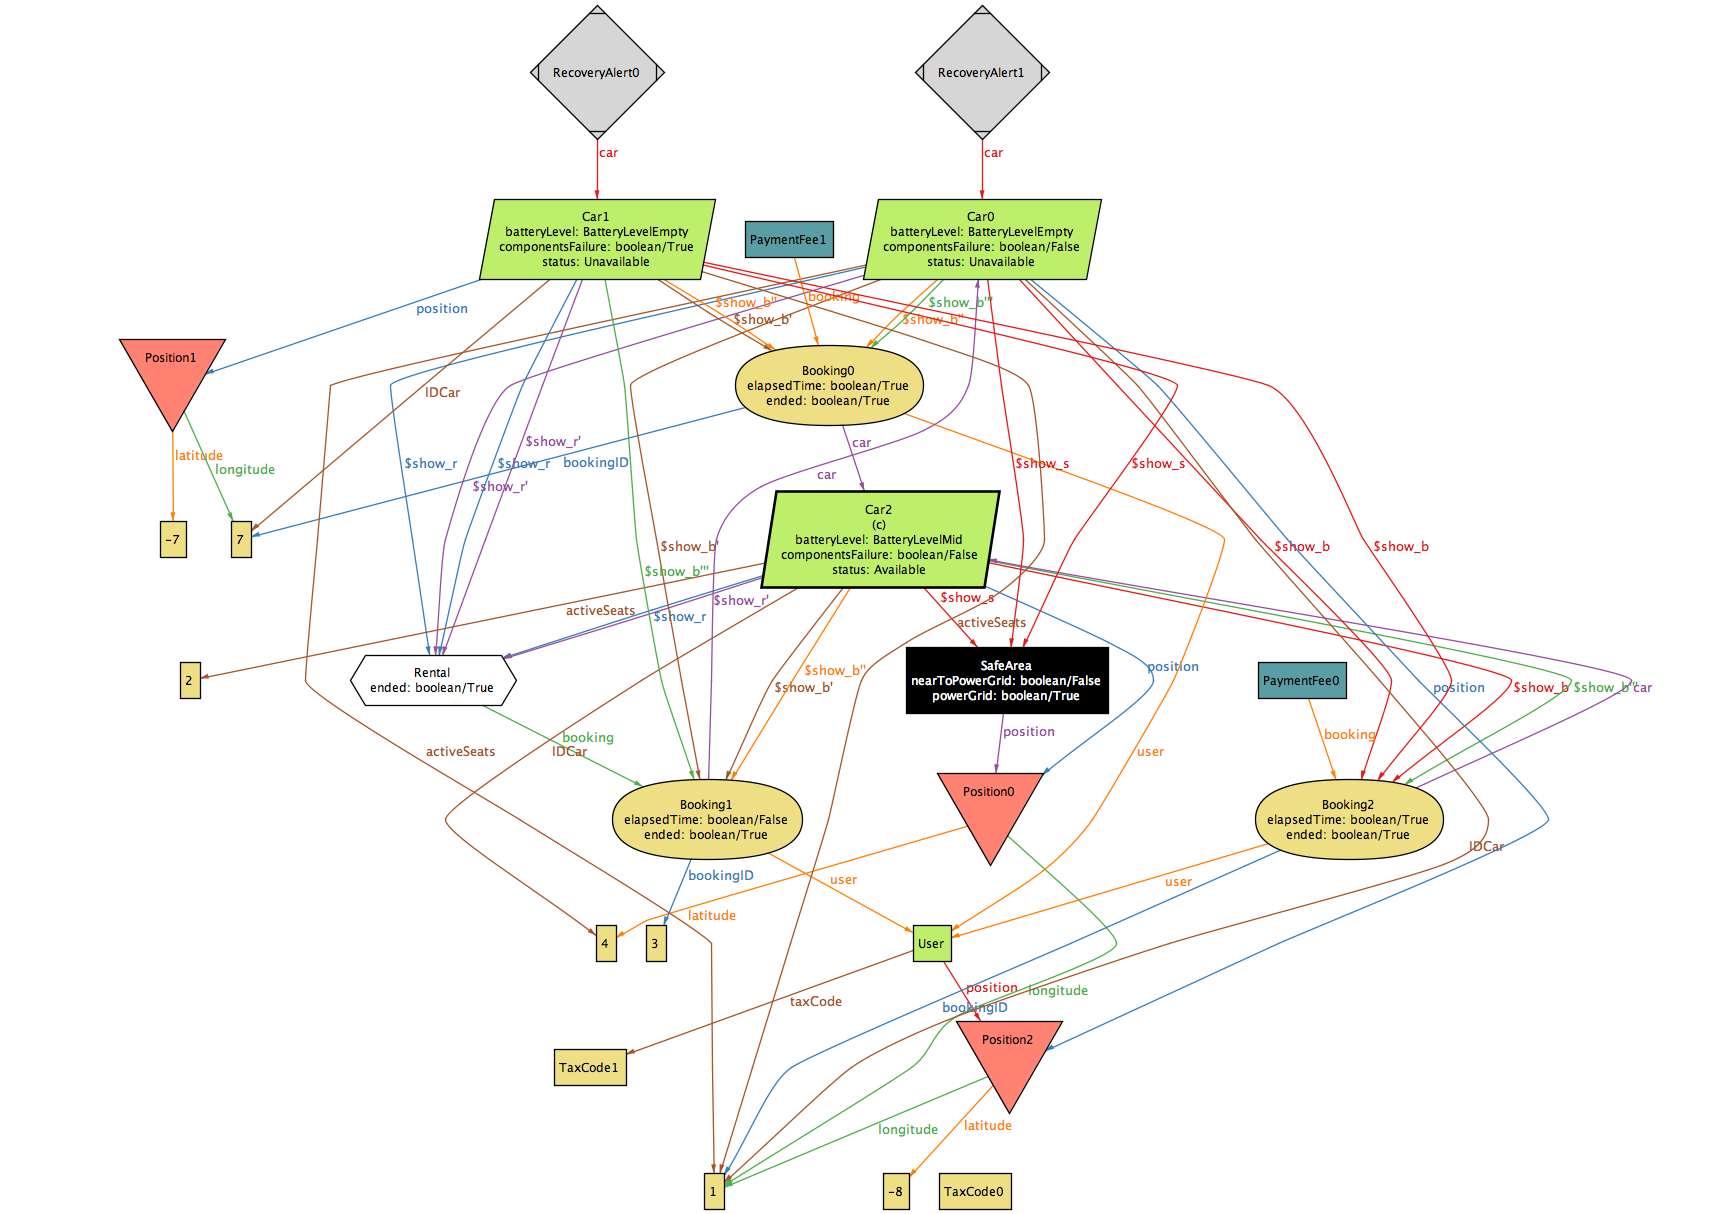
\includegraphics[width=1.425\textwidth, angle=90]{pred-show}
	\caption[Predicate instance - Show]{The image above is a the instance generated by the Alloy Analyzer 4.2 after running the predicate 'show'.}
	\label{fig:pred-show}
\end{figure}

\newpage

\begin{figure}[H]
	\centering
	\includegraphics[width=1.125\textwidth]{pred-allRentalsHaveNonElapsedBooking}
	\caption[Predicate instance - All rentals have non elapsed booking]{The image above is a the instance generated by the Alloy Analyzer 4.2 after running the predicate 'allRentalsHaveNonElapsedBooking'.}
	\label{fig:pred-allRentalsHaveNonElapsedBooking}
\end{figure}

\newpage

\begin{figure}[H]
	\centering
	\includegraphics[width=1.5\textwidth, angle=90]{pred-batteryLowInSafeAreaWithNoPowerGridHasAlert}
	\caption[Predicate instance - Battery low in safe area with no power grid has alert]{The image above is a the instance generated by the Alloy Analyzer 4.2 after running the predicate 'batteryLowInSafeAreaWithNoPowerGridHasAlert'.}
	\label{fig:pred-batteryLowInSafeAreaWithNoPowerGridHasAlert}
\end{figure}

\newpage

\begin{figure}[H]
	\centering
	\includegraphics[width=1.5\textwidth, angle=90]{pred-bookingsElapsedHaveFeePayments}
	\caption[Predicate instance - Bookings elapsed have fee payments]{The image above is a the instance generated by the Alloy Analyzer 4.2 after running the predicate 'bookingsElapsedHaveFeePayments'.}
	\label{fig:pred-bookingsElapsedHaveFeePayments}
\end{figure}


\end{appendices}

\listoffigures
\begingroup
\let\clearpage\relax
%\listoftables
\endgroup

\bibliographystyle{unsrt}
\bibliography{ref}

\end{document}
